\section{Surface models}
\label{sec:surfaces}

\subsection{Validation year}

\Cref{tab:models} compares every model on SPX 2022. The eSSVI mixture fits closest, with
\mixInVal{} of its model IVs inside the bid-ask and no calendar or butterfly violation on any day,
in the quoted domain or the widened one. Every eSSVI-family fit is arbitrage-free on every day of
every panel, with no failed fits. The per-slice SVI fits and the spline come close on fit but
violate the calendar condition on about a fifth of the widened grid (SVI: \sviCalVal). The
penalized network is nearly as close as the mixture and has the best held-out wings; its penalties
leave \pnnCalVal{} of the grid in calendar violation, and it takes about three times as long to fit
(\pnnTimeVal{} against \mixTimeVal\,s a day). \Cref{fig:tradeoff} shows the trade-off: among
arbitrage-free models, the mixture dominates on both axes, and only models that violate the
conditions extrapolate better.

The wing gap is the price of conditions that are sufficient rather than necessary. On sampled SPX
days the calendar conditions bind at the fitted knots (the wing slope $u_+$ at about half of them,
$\psi/\theta$ at a third to a half of the short-dated ones), while the butterfly bounds do not.
Mixing four components recovers part of the gap: a single eSSVI surface misses the wings by 3.24\vp.
On the synthetic Heston and SSVI panels the mixture's wings are better than the penalized
network's on most days. Network-generated knots (\texttt{nmix4}) keep the guarantee but fit worse
than free knots and are sensitive to initialization; they are used in the cross-day model, where
the network is trained across days.

\begin{table}[t]
  \centering\small
  \caption{Surface models on SPX 2022, the validation year (52 days). Quote columns are IV RMSE in
  vol points on fitted quotes, held-out interior strikes and held-out wings, and the share of model
  IVs inside the bid-ask; violations are shares of a dense grid over the quoted domain widened by
  50\% on each side; the last column is fitting time per day. Best values in bold.}
  \label{tab:models}
  \begin{tabular}{lrrrrrrr}
\toprule
& \multicolumn{4}{c}{quotes (RMSE in vp)} & \multicolumn{2}{c}{violations} & \\
\cmidrule(lr){2-5}\cmidrule(lr){6-7}
model & fit & in spread & strikes & wings & calendar & butterfly & s/day \\
\midrule
SSVI & $0.793$ & 22\% & $0.802$ & $3.80$ & 0 & 0 & $0.21$ \\
SVI (per slice) & $0.204$ & 62\% & $0.218$ & $5.07$ & 21.89\% & 7.91\% & $6.86$ \\
smoothing spline & $0.134$ & 64\% & $0.143$ & $3.95$ & 21.61\% & 0.14\% & $<0.01$ \\
MLP, no penalty & $0.341$ & 45\% & $0.344$ & $1.98$ & 20.04\% & 2.50\% & $18$ \\
penalized network (\texttt{pnn}) & $0.125$ & 75\% & $0.124$ & $\mathbf{0.86}$ & 0.38\% & 0.12\% & $109$ \\
eSSVI & $0.419$ & 40\% & $0.421$ & $3.24$ & 0 & 0 & $3.02$ \\
eSSVI mixture (\texttt{mix4}) & $\mathbf{0.121}$ & \textbf{81\%} & $\mathbf{0.123}$ & $1.31$ & 0 & 0 & $33$ \\
network-generated mixture & $0.406$ & 49\% & $0.407$ & $1.79$ & 0 & 0 & $62$ \\
conditional, amortized & $0.805$ & 16\% & $0.801$ & $1.86$ & 0 & 0 & $0.06$ \\
conditional, refined & $0.610$ & 21\% & $0.615$ & $2.20$ & 0 & 0 & $3.55$ \\
\bottomrule
\end{tabular}

\end{table}

\begin{figure}[t]
  \centering
  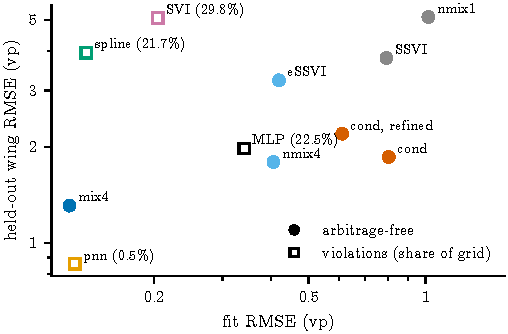
\includegraphics[width=0.6\linewidth]{tradeoff.pdf}
  \caption{Fit against wing extrapolation on SPX 2022 (both log scales). Filled markers are
  arbitrage-free on the whole widened grid; open markers violate it, with the calendar plus
  butterfly violation share in parentheses.}
  \label{fig:tradeoff}
\end{figure}

\subsection{Test year and replication window}

\Cref{tab:oos} reports the same metrics on SPX 2023 and on 2016--2017. On 2023 only the mixture and
the conditional models were scored. The mixture again fits closest (\mixFitTest\vp). The conditional
model trained on 2010--2021 and refitted before each quarter is the best on the wings
(\condWingTest{} against \mixWingTest\vp). That run was the third on 2023, and the wing gain is
uneven: the refitted model is better on only 27 of the 50 days. On 2016--2017, which no choice was
tuned on, every model was scored once with the settings chosen on 2022. The rankings of 2022 hold:
the mixture fits closest and is arbitrage-free (\mixFitRep\vp, \mixInRep{} inside the bid-ask), the
penalized network has the best wings (\pnnWingRep\vp) with a few violations left, and SVI and the
spline violate the calendar condition. One 2023 finding does not replicate: the walk-forward
conditional model trails the mixture on the wings (\condWingRep{} against \mixWingRep\vp). Every
model sits inside the bid-ask more often than in 2022, because spreads were wider (median
half-spreads of 0.14--0.20 against 0.10\vp).

\begin{table}[t]
  \centering\small
  \caption{Surface models on the test year and on the replication window; columns as in
  \cref{tab:models}. On 2023 only the mixture and the conditional models were scored. ``Frozen''
  models stop training at the end of their training years; ``walk-forward'' copies are fine-tuned
  before each quarter on every day up to its start.}
  \label{tab:oos}
  \begin{tabular}{lrrrrrrr}
\toprule
& \multicolumn{4}{c}{quotes (RMSE in vp)} & \multicolumn{2}{c}{violations} & \\
\cmidrule(lr){2-5}\cmidrule(lr){6-7}
model & fit & in spread & strikes & wings & calendar & butterfly & s/day \\
\midrule
\multicolumn{8}{l}{\emph{SPX 2023, test year (50 days)}} \\
eSSVI mixture (\texttt{mix4}) & $\mathbf{0.071}$ & \textbf{80\%} & $\mathbf{0.076}$ & $0.82$ & 0 & 0 & $26$ \\
conditional, 2018--2021, frozen & $0.610$ & 13\% & $0.611$ & $1.44$ & 0 & 0 & $0.05$ \\
conditional, 2018--2021, walk-forward & $0.397$ & 20\% & $0.397$ & $0.85$ & 0 & 0 & $0.05$ \\
conditional, 2010--2021, frozen & $0.476$ & 17\% & $0.478$ & $1.25$ & 0 & 0 & $0.08$ \\
conditional, 2010--2021, walk-forward & $0.376$ & 19\% & $0.377$ & $\mathbf{0.70}$ & 0 & 0 & $0.08$ \\
\quad the same, refined & $0.323$ & 25\% & $0.324$ & $0.78$ & 0 & 0 & $1.90$ \\
\midrule
\multicolumn{8}{l}{\emph{SPX 2016--2017, replication (101 days)}} \\
SSVI & $0.614$ & 37\% & $0.622$ & $1.83$ & 0 & 0 & $0.12$ \\
SVI (per slice) & $0.128$ & 90\% & $0.138$ & $2.67$ & 15.64\% & 10.92\% & $8.39$ \\
smoothing spline & $0.130$ & 83\% & $0.147$ & $2.23$ & 7.43\% & 0.66\% & $<0.01$ \\
penalized network (\texttt{pnn}) & $0.085$ & 96\% & $0.086$ & $\mathbf{0.32}$ & 0.08\% & 0.00\% & $194$ \\
eSSVI mixture (\texttt{mix4}) & $\mathbf{0.068}$ & \textbf{99\%} & $\mathbf{0.071}$ & $0.35$ & 0 & 0 & $32$ \\
conditional, 2010--2015, frozen & $0.512$ & 34\% & $0.507$ & $0.75$ & 0 & 0 & $0.11$ \\
conditional, 2010--2015, walk-forward & $0.375$ & 43\% & $0.373$ & $0.55$ & 0 & 0 & $0.07$ \\
\quad the same, refined & $0.289$ & 55\% & $0.288$ & $0.52$ & 0 & 0 & $1.56$ \\
\bottomrule
\end{tabular}

\end{table}

\subsection{Regime change limits the cross-day model on SPX}

On SPX 2022 the conditional model fits five to seven times worse than the mixture
(\cref{tab:models}), because 2022 left the family of surfaces it learned. Its amortized error is
\condQIn--\condQInMax\vp{} in every sampled quarter of 2019 and 2021, but \condQOne\vp{} in 2022Q1 and
\condQFour\vp{} by 2022Q4, while the ATM skew $\partial\sigma/\partial k$ flattens from $\skewQOne$
to $\skewQFour$ (\cref{fig:regime}). Neither the encoder nor the maturity grid is the cause:
thinning the extra short-dated expiries of 2022 back to the training count leaves the error
unchanged, the mixture restricted to the decoder's maturity grid still fits 2022 to 0.19--0.29\vp,
and refining the latent recovers only 3--11\% of the error. Walk-forward refits close about half of
the 2022 gap, and training from 2010 lowers the error everywhere (\cref{tab:oos}), but the frozen
model's 2022 error stays twice its early-stopping error, so 2022 also lies outside 2010--2021.

\begin{figure}[t]
  \centering
  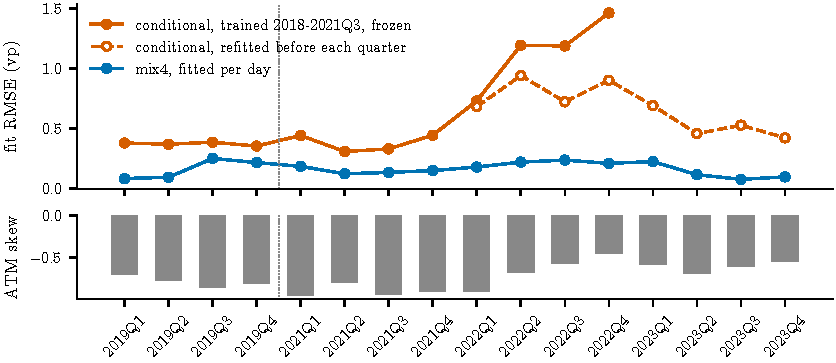
\includegraphics[width=\linewidth]{regime.pdf}
  \caption{Amortized fit error of the conditional model by quarter on the evaluation days, frozen
  after training on 2018--2021Q3 and refitted before each quarter, against the per-day mixture; the
  lower panel is the quarter's ATM skew $\partial\sigma/\partial k$. 2020 was not sampled (dotted line).}
  \label{fig:regime}
\end{figure}

\subsection{Missing strikes and maturities}

\Cref{fig:gaps} refits every model with more of each chain held out. On SPX the per-day mixture
degrades slowly and stays best: with 90\% of interior strikes held out it misses them by
\mixGapNinety\vp, against \sviGapNinety{} for SVI and \condGapNinety{} for the refined conditional
model. With 30\% of inner maturities held out it misses by \mixGapSlices\vp, against \condGapSlices{}
for the conditional model and \sviGapSlices{} for SVI, which also violates calendar arbitrage there.
The conditional model's error barely moves with the share held out, on both panels, and on Heston it
is best at every level: with 90\% of strikes missing its error against the true surface is
\hestonTruthNinetyCond\vp, against \hestonTruthNinetyMix{} for the mixture. At 90\% SVI cannot fit any
Heston day, because too few strikes remain per slice.

\begin{figure}[t]
  \centering
  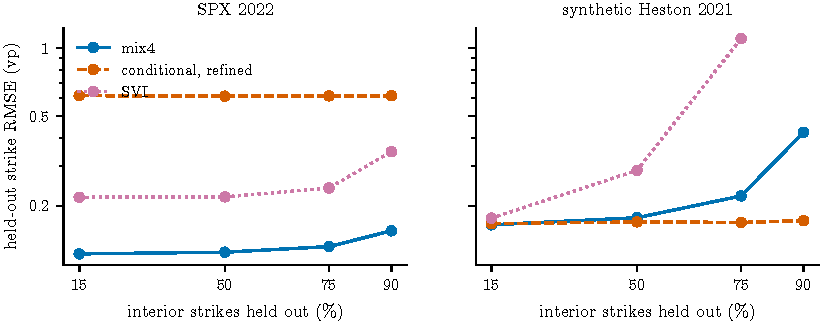
\includegraphics[width=\linewidth]{gaps.pdf}
  \caption{Error on held-out interior strikes as more of each chain is held out (log scale); every
  model is refitted at each level. SVI cannot fit a Heston day with 90\% held out.}
  \label{fig:gaps}
\end{figure}

\subsection{Synthetic panels: the cross-day model wins}

On synthetic Heston, whose regime does not change between years, the cross-day model is the best
surface model (\cref{tab:heston}). Trained on one year, it already beats the mixture against the
truth on the validation year, but its amortized error rises by 70--80\% on the test years, whose
variance falls below anything in its training year. Trained on nine generator years, it is less than half as far from
the true surface as the mixture on every panel, with the closest wings and \multiInFresh{} of its
model IVs inside the bid-ask, in an \multiTime\,ms forward pass against \mixTimeHeston\,s. The
mixture stays closest to the quotes themselves, because it also fits each day's quote noise.

\begin{table}[t]
  \centering\small
  \caption{Error against the true surface on synthetic Heston (vp): held-out interior strikes and
  held-out wings, on the validation year, the test year and a fresh test panel generated with a new
  seed. The conditional model is trained on one year (2020) or on nine.}
  \label{tab:heston}
  \begin{tabular}{lrrrrrr}
\toprule
& \multicolumn{3}{c}{held-out strikes} & \multicolumn{3}{c}{held-out wings} \\
\cmidrule(lr){2-4}\cmidrule(lr){5-7}
model & 2021 (val.) & 2022 (test) & fresh 2023 & 2021 & 2022 & fresh 2023 \\
\midrule
eSSVI mixture (\texttt{mix4}) & $0.094$ & $0.098$ & $0.099$ & $0.248$ & $0.254$ & $0.244$ \\
conditional, one year & $0.083$ & $0.138$ & $0.152$ & $0.138$ & $0.187$ & $0.222$ \\
\quad refined & $0.062$ & $0.078$ & $0.082$ & $0.145$ & $0.159$ & $0.173$ \\
conditional, nine years & $0.040$ & $0.045$ & $0.045$ & $\mathbf{0.112}$ & $\mathbf{0.109}$ & $\mathbf{0.127}$ \\
\quad refined & $\mathbf{0.040}$ & $\mathbf{0.040}$ & $\mathbf{0.042}$ & $0.128$ & $0.120$ & $0.135$ \\
\bottomrule
\end{tabular}

\end{table}

\subsection{Forecasting}

No model forecasts the surface better than a random walk (\cref{tab:forecast} in
\cref{app:forecast}). On SPX the latent
VAR loses to the origin day's mixture surface at one day ($p<0.001$), because the decoded surface's
own 2022 error (last column) is almost as large as a one-day move. At 20 days its error is lower
(\fcVarTwenty{} against \fcRwTwenty\vp), but not significantly ($p=\fcPTwenty$). The Heston panel is
the positive control. The latent encodes the true log-variance almost linearly (out-of-sample
$R^2=0.995$), and forecasting that state with the generator's own dynamics beats the random walk by
24\% at 20 days ($p=0.03$). An AR(1) fitted to the true state over the single training year, however,
loses by 80\%, and the latent VAR by a similar margin: one year of a process with a 35-day half-life
is too short to estimate its mean. The representation carries the forecastable signal, but its
dynamics cannot be estimated from one year.
